\documentclass[presentation]{subfiles}

\begin{document}

\section{Complexity}

\begin{frame}{Complexity}
  What kinds of problems do we mean when we talk about complexity?
  \begin{mystepwiseitemize}
    \item Can crowds improve existing works?~\cite{bernsteinSoylent,Kim:2014:CSI:2556288.2556986}
    \item Can crowds critique designs?~\cite{yuanAlmost}
    \item Can crowds create things from whole cloth?~\cite{KimStoria,Kim2017,Hahn:2016:KAB:2858036.2858364,Lasecki:2014:LSR:2661334.2661352}
  \end{mystepwiseitemize}
\end{frame}


\begin{frame}{What does the crowdsourcing literature say?}
\begin{columns}
  \begin{column}{0.5\textwidth}
    \begin{itemize}
      \item Build complexity into the process
      \begin{mystepwiseitemize}
        \item Apply CS methods to people~(\textcite{crowdForgeKittur})
        \item see other stuff
      \end{mystepwiseitemize}
    \end{itemize}
  \end{column}
  
  \begin{column}{0.5\textwidth}
    \begin{figure}
    % \visible<2>{
    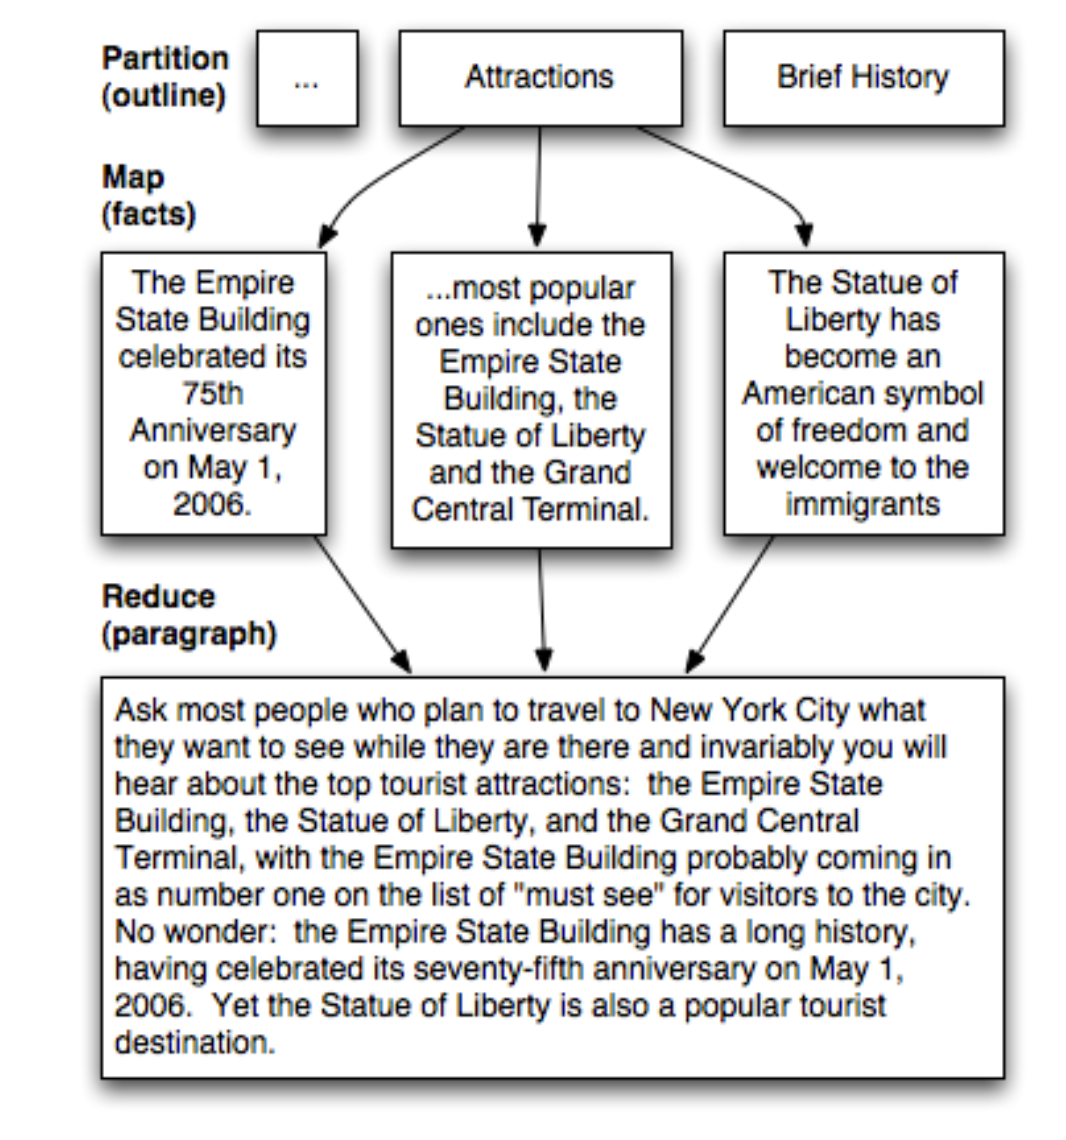
\includegraphics[width=0.7\textwidth]{figures/mapReduce.png}
    % }
    % \visible<1>{

    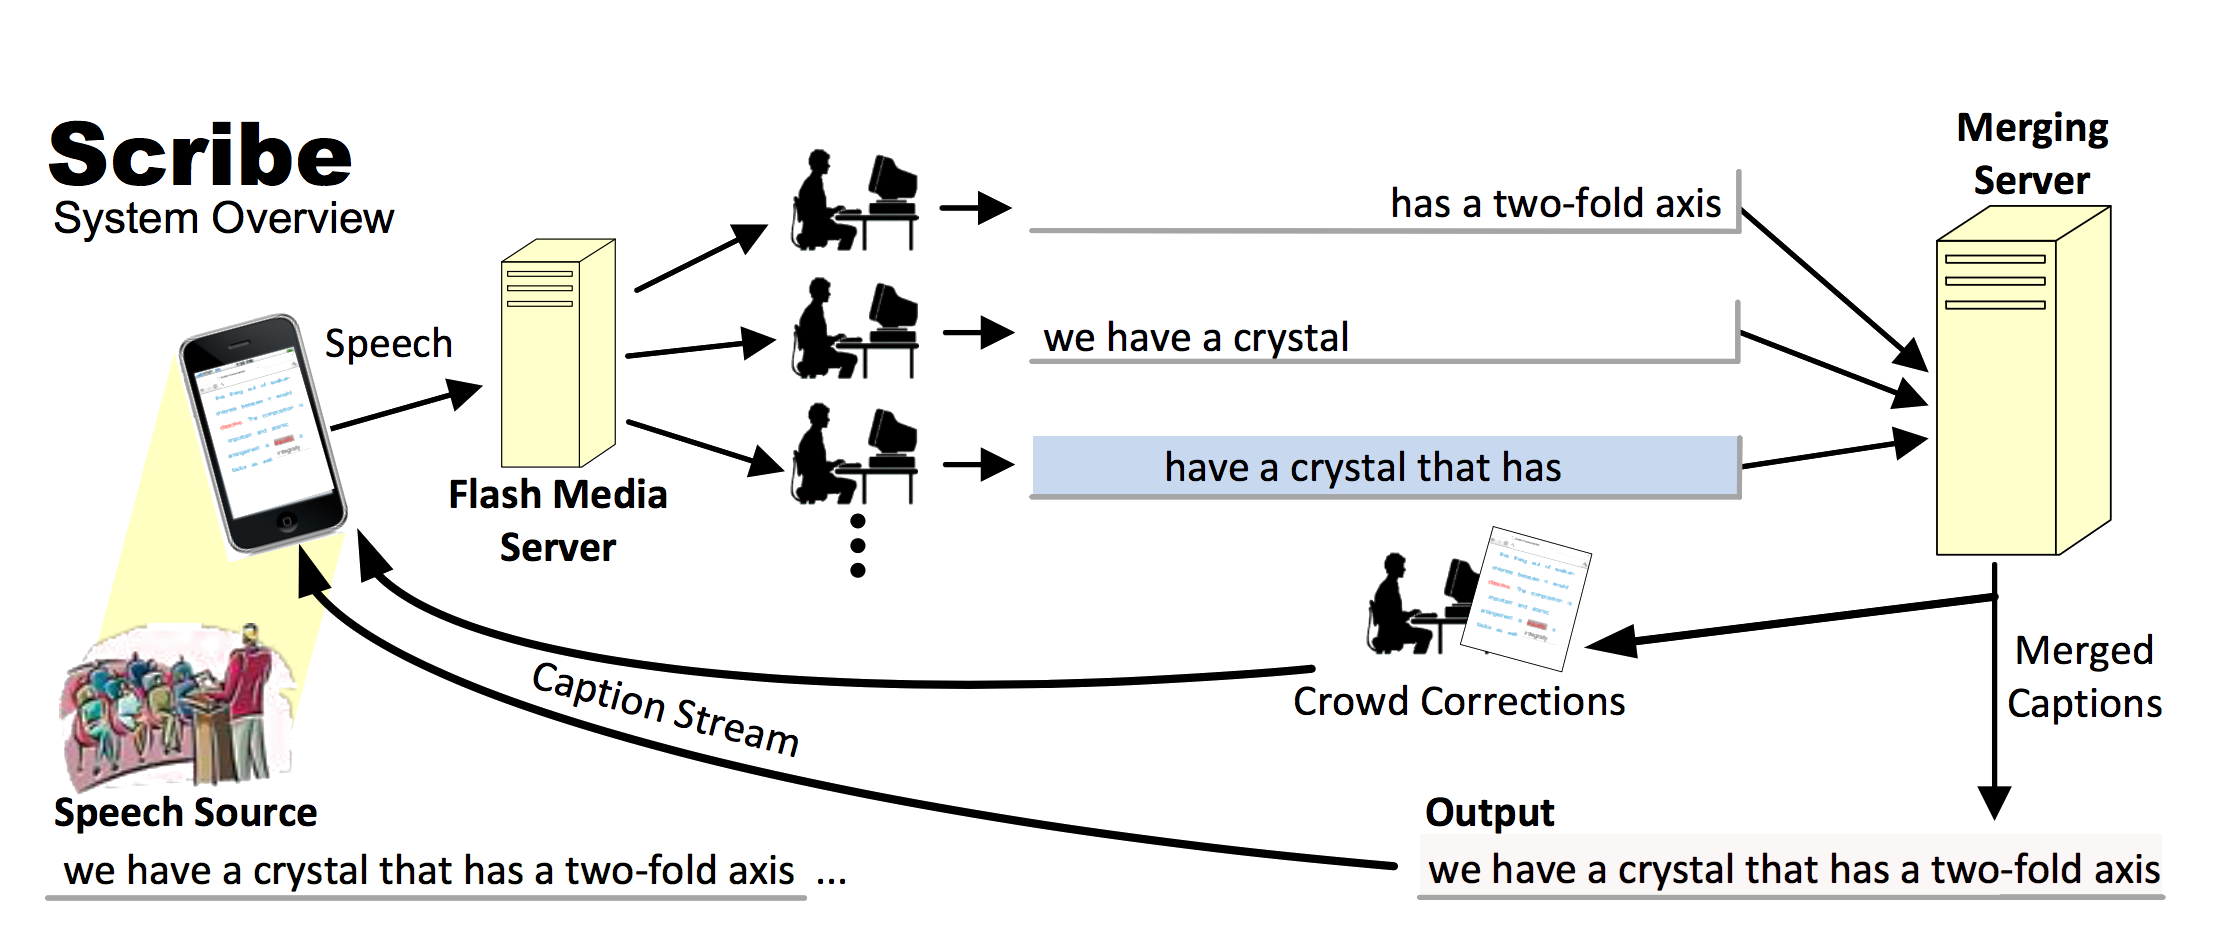
\includegraphics[width=0.7\textwidth]{figures/complexity/cw_literature/scribe.png}
    % }
    \end{figure}
  \end{column}
  
\end{columns}
\end{frame}

\begin{frame}{What does the piecework literature say?}
    something even more insightful, I'm sure!
\end{frame}

\begin{frame}{Comparisons}
% \framesubtitle{something else}
%   \begin{columns}
%   \begin{column}{0.5\textwidth}
%   % \section*{Piecework}
%      some text here some text here some text here some text here some text here

%   \end{column}

%   \begin{column}{0.5\textwidth}
%   % \section*{CrowdWork}
%      some text here some text here some text here some text here some text here

%   \end{column}
%   \end{columns}
\end{frame}
\end{document}